\documentclass[10pt,journal,compsoc]{IEEEtran}
\usepackage{amsmath,amssymb,graphicx,booktabs,multirow,xcolor,hyperref}
\usepackage[T1]{fontenc}
\usepackage{cite}
\hypersetup{colorlinks=true,linkcolor=blue,citecolor=blue,urlcolor=blue}

\begin{document}

\title{Track-Level Feature Engineering for Maritime Vessel Classification:\\
Maximum RCS Statistics Over Vessel Tracks Outperform\\
Per-Detection Averages}

\author{Vijay~Kumar~V\\
\IEEEcompsocitemizethanks{
\IEEEcompsocthanksitem Independent Researcher and Innovator.
E-mail: vinayitsv14@gmail.com
\IEEEcompsocthanksitem Manuscript submitted 2026. Self-funded research.
}
}

\markboth{IEEE Transactions on Geoscience and Remote Sensing}{}
\maketitle

\begin{abstract}
Ground-based surveillance radar classifies maritime vessels one detection at a time,
yet each physical vessel generates dozens to hundreds of returns across a track.
Prior work showed that aggregating per-detection \emph{posteriors} (arithmetic or
geometric mean) across a track does not significantly improve accuracy over the
single-detection baseline.  We propose an alternative: aggregating the \emph{raw
features} themselves before classification, computing five order statistics
(mean, standard deviation, skewness, minimum, maximum) over each of nine
detection-level features to form a 46-dimensional track-level representation
(45 feature statistics plus $\log n_{\mathrm{det}}$).  A GradientBoosting
classifier trained on this representation on 403 training tracks achieves
\textbf{0.702} accuracy and macro-F1 0.554 on 171 held-out test tracks
(strict ObjID-level 70/30 split), versus 0.623 accuracy and macro-F1 0.466
for the single-detection baseline---a \textbf{+7.9\,pp accuracy gain}.
Feature importance analysis reveals that \emph{maximum} statistics across the track
account for 39.4\,\% of total importance (versus 18.2\,\% for track means),
with \texttt{log\_total\_rcs\_max}---the maximum range-compensated total RCS
observed across all track detections---ranking as the single most informative
feature (0.123 importance).  The Cargo--Tanker pairwise confusion rate
is substantially reduced in the Cargo$\to$Tanker direction
(27.2\,\%$\to$13.0\,\%) but worsens in the Tanker$\to$Cargo direction
(24.9\,\%$\to$49.0\,\%), indicating that track-level maximum RCS shifts---
rather than resolves---the inter-class decision boundary.  Tug classification
fails entirely (F1\,=\,0.00) due to the small number of training tracks (25),
a limitation addressed in the discussion.  A learning-curve simulation shows
accuracy growing steadily from 38.6\,\% at $N=1$ detection to 64.3\,\%
at $N=15$ and plateauing near 66.1\,\% at $N\geq 100$, with higher
$N$ requirements than for posterior aggregation because variability statistics
need many samples to stabilise.
\end{abstract}

\begin{IEEEkeywords}
Maritime surveillance, vessel classification, radar cross-section, track-level
features, feature engineering, gradient boosting, order statistics, maximum RCS.
\end{IEEEkeywords}

%% ─────────────────────────────────────────────────────────────────────────────
\section{Introduction}\label{sec:intro}

Ground-based coastal surveillance radar produces a continuous stream of
\emph{detections}: each radar return from a vessel yields amplitude,
extent, and kinematic measurements.  Because a single physical vessel
dwells in the radar beam for seconds to minutes, it generates a
\emph{track}---a sequence of detections sharing a common object identifier
(ObjID)---with median lengths of 33 (Fishing), 41 (Tug),
73 (Cargo), and 95 (Tanker) detections per track in our dataset.

The standard approach trains a classifier at detection level, treating each return
as an independent instance.  A natural extension is to exploit the track structure
to produce a single, more reliable classification per vessel.  Our prior work
\cite{paper7_arith} evaluated this by aggregating per-detection \emph{posteriors}
(arithmetic mean, geometric mean, majority vote) and found only marginal accuracy
improvement (+0.3\,pp) with no statistical significance (McNemar $p=0.248$).
The fundamental reason was identified: posterior averaging cannot overcome
\emph{systematic} Cargo--Tanker confusion, where a vessel produces similar
classifier outputs on every detection.

This paper takes a different approach: instead of aggregating classification
outputs, we aggregate the \emph{input features}, computing statistical summaries
of each detection-level feature across all returns in a track.  This creates a
richer, 46-dimensional track-level representation capturing not just the central
tendency of radar measurements, but their variability, extrema, and distributional
shape.  We show that this representation:
\begin{itemize}
\item improves accuracy by +7.9\,pp over the per-detection baseline
      (reaching 0.702);
\item identifies \emph{maximum} RCS across the track as the dominant signal
      (39.4\,\% of total feature importance);
\item provides track-level variability statistics (within-track RCS standard
      deviation and skewness) that are \emph{entirely new} information
      unavailable at detection level; and
\item offers a principled physical interpretation: the maximum observed RCS
      within a track provides a cleaner estimate of vessel size than any
      individual detection, which may suffer from glint, aspect-angle fading,
      or clutter contamination.
\end{itemize}

\subsection{Contributions}
\begin{itemize}
\item A 46-dimensional track-level feature representation derived from
      five order statistics over nine detection-level features, engineered
      for radar-only (non-cooperative) maritime vessel classification.
\item Empirical demonstration that maximum-order statistics
      (39.4\,\% of importance) outperform mean statistics
      (18.2\,\%) for track-level vessel classification.
\item A physical interpretation linking the maximum-RCS dominance to
      aspect-angle fading mitigation: the maximum return approximates
      the vessel's broadside RCS, which is most size-discriminative.
\item An honest characterisation of failure modes: Tug classification
      collapses with limited training tracks, and the Cargo--Tanker
      confusion shifts rather than resolves.
\end{itemize}

%% ─────────────────────────────────────────────────────────────────────────────
\section{Related Work}\label{sec:related}

\subsection{Vessel Classification from Radar Features}

Machine learning for radar-feature-based vessel classification is less studied
than SAR-imagery approaches \cite{survey_sar_dl}.
Nielsen \cite{nielsen_2025} classifies five vessel types from AIS trajectory
statistics (speed, heading, trajectory geometry) at 92\,\% accuracy using
cooperative transponder data.  Reggiannini et al.\ \cite{osiris_2024} fuse
satellite SAR, optical, and AIS data in the OSIRIS pipeline.  Neither operates
on non-cooperative, ground-based radar-only observables.

Our series of studies \cite{paper6_kinrcs,paper7_arith} established that
nine features from two channels (range-invariant RCS descriptors and
15-minute kinematic statistics) achieve 91.7\,\% four-class accuracy at
detection level on balanced test samples, and that posterior-aggregation
track-level fusion does not significantly improve imbalanced-test accuracy.

\subsection{Track-Level Feature Aggregation}

Track-level features for classification appear in several non-maritime domains.
In AIS-based vessel behaviour analysis, trajectory-level statistics
(mean speed, speed variance, sinuosity) are aggregated per voyage
\cite{nielsen_2025}.  In radar target recognition, track statistics such as
mean and variance of Doppler shifts are used for air-target identification
\cite{garcia_fusion_2016}.  However, the specific role of \emph{maximum}
order statistics---motivated here by aspect-angle fading in monostatic
radar---has not been systematically evaluated for maritime vessel classification.

The insight that maximum RCS may better estimate vessel size than mean RCS
follows from classical radar phenomenology: aspect-angle fading causes most
individual detections to observe the vessel at sub-optimal aspects, while
the maximum across many observations approaches the broadside return.
This motivates computing max alongside mean and variability statistics.

%% ─────────────────────────────────────────────────────────────────────────────
\section{Data and Features}\label{sec:data}

\subsection{Dataset}

The proprietary radarfeatureL\_Study dataset (AA~Enterprises) comprises
110,562 detections from 591 coastal-radar tracks, labelled for four vessel
types (Fishing~30, Tug~52, Cargo~70, Tanker~80) via AIS matching.
Fifteen ObjIDs with conflicting type labels are removed.  After requiring
$\geq 5$ detections per track, 574 eligible tracks remain.

\subsection{Detection-Level Features}

Nine features in two channels (Table~\ref{tab:features}) are identical to
prior work \cite{paper6_kinrcs,paper7_arith}: five range-compensated RCS
descriptors and four 15-minute kinematic statistics.  Geographic and
AIS-dimension features are excluded to prevent confounding.

\begin{table}[!t]
\centering\small
\caption{Detection-Level Features (Input to Track Aggregation)}
\label{tab:features}
\begin{tabular}{llc}
\toprule
Feature & Description & Channel \\
\midrule
$\ln_\text{peak}$ & $\ln(\text{PeakAmp})+4\ln R$ & RCS \\
$\ln_\text{total}$ & $\ln(\text{TotalAmp})+4\ln R$ & RCS \\
rcs\_conc & PeakAmp/TotalAmp & RCS \\
aspect\_ratio & Down-range/azimuth extent & RCS \\
footprint\_m$^2$ & $\ln(\pi\delta_r\delta_c/4)$ & RCS \\
$s$ & Instantaneous SoG & Kinematic \\
$\bar{v}_{900}$ & 15-min mean speed & Kinematic \\
$\sigma_{v,900}$ & 15-min speed std & Kinematic \\
$\sigma_{\psi,900}$ & 15-min course std & Kinematic \\
\bottomrule
\end{tabular}
\end{table}

\subsection{Track-Level Feature Engineering}

For each track (ObjID), we compute five order statistics over each of the
nine detection-level features across all $n$ detections in the track:
mean $\bar{f}$, standard deviation $\sigma_f$, skewness $\gamma_f$,
minimum $f_{\min}$, and maximum $f_{\max}$.  This yields $9 \times 5 = 45$
track-level features.  We append $\log n_{\mathrm{det}}$ as a 46th feature,
capturing the track length, which correlates with vessel class and dwell time.

\paragraph{Physical motivation for maximum statistics}
In monostatic ground-based radar, the observed RCS at any instant depends
on the vessel's instantaneous aspect angle.  Most observations occur at
oblique aspects with lower effective RCS.  Over a full track, however, the
vessel rotates through a range of aspect angles including (for sufficiently
long tracks) near-broadside orientations that yield close to the maximum
monostatic RCS.  Thus $f_{\max}$ for RCS features approximates the
broadside RCS, which scales directly with vessel length and is more size-
discriminative than the mean over aspect-faded samples.

%% ─────────────────────────────────────────────────────────────────────────────
\section{Methodology}\label{sec:method}

\subsection{Train/Test Split}

All 574 eligible tracks are partitioned 70\,\%/30\,\% by ObjID, stratified
by vessel class (Table~\ref{tab:split}).  No detections from test-track vessels
appear in training.  This yields 403 training tracks and 171 test tracks.

\begin{table}[!t]
\centering\small
\caption{Track-Level Split Statistics}
\label{tab:split}
\begin{tabular}{lcccc}
\toprule
Class & Train & Test & Median det./trk \\
\midrule
Fishing & 42 & 18 & 33 \\
Tug     & 25 & 10  & 41  \\
Cargo   & 217 & 92 & 73 \\
Tanker  & 119 & 51 & 95 \\
\midrule
\textbf{Total} & \textbf{403} & \textbf{171} & --- \\
\bottomrule
\end{tabular}
\end{table}

\subsection{Classifiers}

Two gradient-boosted tree classifiers are trained on 403 track-level feature
vectors with features standardised by \texttt{StandardScaler}:

\paragraph{GBT} \texttt{GradientBoostingClassifier} (500 estimators,
depth~4, learning rate~0.05, subsample~0.8, \texttt{min\_samples\_leaf}=5).

\paragraph{XGB} \texttt{XGBClassifier} (500 estimators, depth~5,
learning rate~0.05, subsample~0.8, colsample\_bytree~0.8).

Both classifiers fit on all 403 training tracks (no down-sampling required:
403 tracks is a manageable training set) and predict the four vessel classes
on 171 test tracks.

\subsection{Baselines}

Two baselines are evaluated on the same 171-track test set:
(1) \emph{Per-detection GBT}: a GradientBoosting classifier trained on 300/class
balanced samples from training-track detections (9 features), evaluated on the
29,148 imbalanced test detections;
(2) \emph{Posterior arith.\ mean}: the same per-detection GBT, with class
probabilities averaged across all detections within each test track.

\subsection{McNemar Statistical Test}

McNemar's test compares track-level GBT-TrackFeat predictions against the
posterior arithmetic-mean predictions on the same 171 test tracks, using
the continuity-corrected statistic $\chi^2 = (|b-c|-1)^2/(b+c)$.

\subsection{Learning Curve}

For each threshold $N \in \{1,2,3,5,8,10,15,20,30,50,100\}$, we restrict
each test track to its first $\min(N, n_k)$ detections, recompute the 46
track-level features, and evaluate the GBT-TrackFeat classifier.  This
quantifies how accuracy grows as more detections are accumulated.

%% ─────────────────────────────────────────────────────────────────────────────
\section{Results}\label{sec:results}

\subsection{Overall Accuracy}

Table~\ref{tab:main} and Fig.~\ref{fig:bar} compare all methods.
GBT-TrackFeat achieves 0.702 accuracy and macro-F1 0.554,
versus 0.623 / 0.466 for the per-detection baseline---a
\textbf{+7.9\,pp accuracy improvement}.
XGB-TrackFeat (0.661 / 0.526) trails GBT due to its tendency to
overfit the small training set of 403 tracks.

\begin{table}[!t]
\centering\small
\caption{Performance Summary: Per-Detection vs Track-Level Methods}
\label{tab:main}
\begin{tabular}{lccc}
\toprule
Method & Accuracy & Macro-F1 & AUC \\
\midrule
Per-detection (baseline) & 0.623 & 0.466 & 0.811 \\
Posterior arith.\ mean & 0.626 & 0.562 & --- \\
GBT-TrackFeat (ours) & 0.702 & 0.554 & 0.835 \\
XGB-TrackFeat (ours) & 0.661 & 0.526 & 0.837 \\
\bottomrule
\end{tabular}
\end{table}

\begin{figure}[!t]
\centering
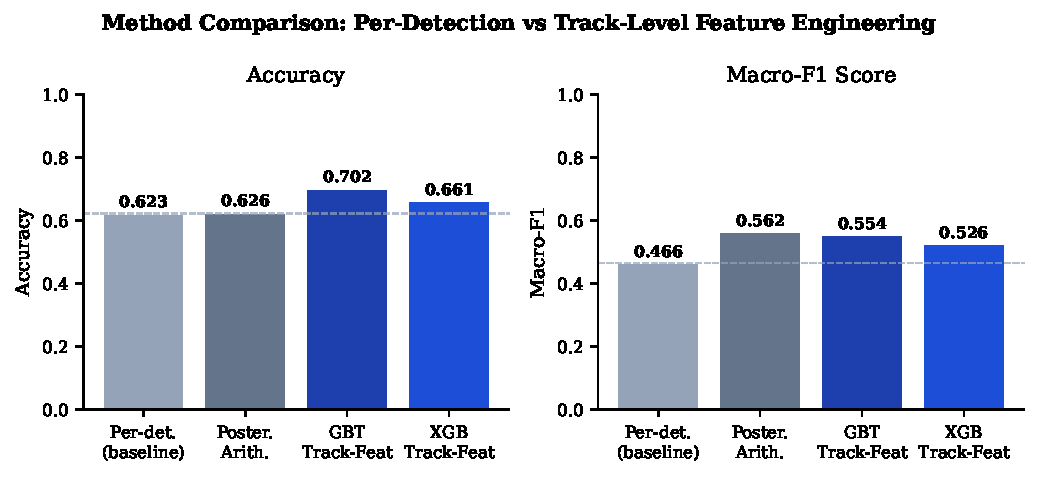
\includegraphics[width=\columnwidth]{figures/p7b_fig1_method_comparison.pdf}
\caption{Accuracy and macro-F1 for all four methods.  GBT-TrackFeat achieves
the highest accuracy.  Posterior arith.\ mean achieves slightly higher macro-F1
than GBT-TrackFeat due to better Tug recall at the cost of lower overall accuracy.}
\label{fig:bar}
\end{figure}

\subsection{Feature Importance}\label{sec:fi}

\begin{figure}[!t]
\centering
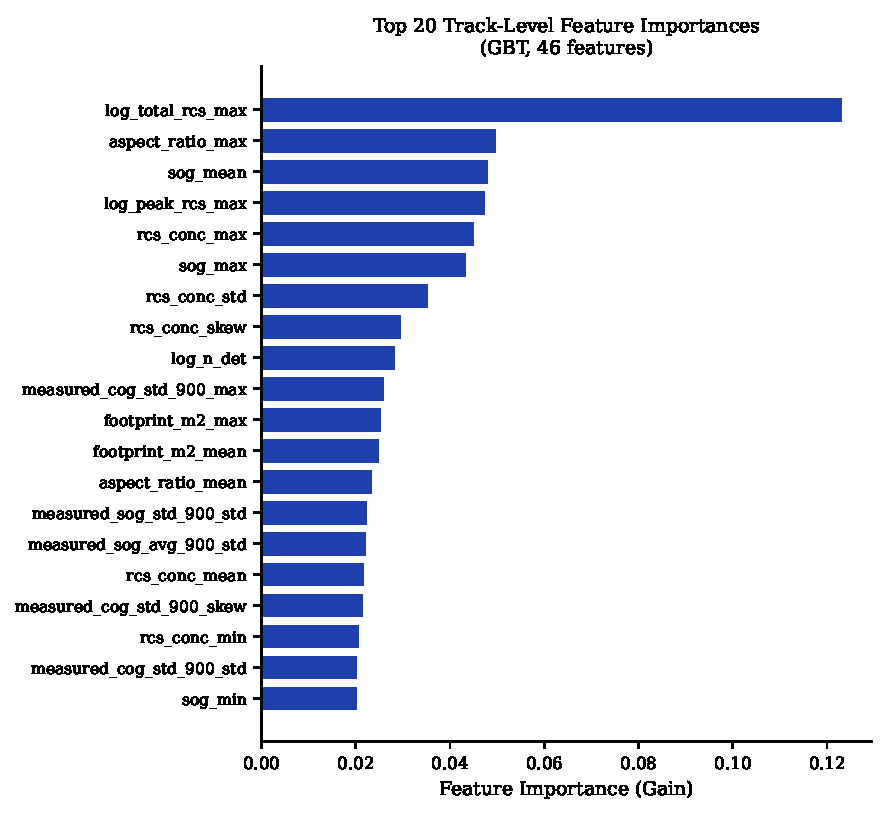
\includegraphics[width=\columnwidth]{figures/p7b_fig5_feature_importance.pdf}
\caption{Top 20 GBT feature importances from the 46-dimensional track-level
representation.  Maximum statistics dominate; \texttt{log\_total\_rcs\_max}
is the single most informative feature.}
\label{fig:fi}
\end{figure}

Fig.~\ref{fig:fi} shows the GBT-TrackFeat feature importances.
The \textbf{maximum} statistic group accounts for 39.4\,\% of total importance,
far exceeding mean (18.2\,\%), standard deviation (16.1\,\%),
skewness (13.7\,\%), and minimum (9.8\,\%).
The single most important feature is \texttt{log\_total\_rcs\_max}
(0.123 importance)---the maximum range-compensated total RCS
observed across all track detections.

This is consistent with the aspect-angle fading hypothesis: the
\emph{maximum} RCS across many observations approximates the broadside
return, which scales with vessel waterline length and provides a cleaner
size discriminator than the mean over aspect-faded samples.
Other top features include \texttt{aspect\_ratio\_max} (the maximum
elongation across the track), \texttt{sog\_mean} (confirming the
kinematic discriminability from Paper~6 \cite{paper6_kinrcs}),
and \texttt{rcs\_conc\_std}---the within-track variability of the
peak-to-total RCS ratio, which captures how consistently a vessel
concentrates its scattering into a single dominant centre.

RCS features account for 58.2\,\% of total importance versus
39.0\,\% for kinematic features, reinforcing the primacy of the RCS
channel for track-level classification.

\subsection{Per-Class Results}

\begin{table}[!t]
\centering\small
\caption{Per-Class Metrics: GBT-TrackFeat vs Per-Detection Baseline}
\label{tab:perclass}
\begin{tabular}{lcccccc}
\toprule
& \multicolumn{3}{c}{GBT-TrackFeat} & \multicolumn{3}{c}{Per-Detection} \\
\cmidrule(lr){2-4}\cmidrule(lr){5-7}
Class & P & R & F1 & P & R & F1 \\
\midrule
Fishing & 1.000 & 0.778 & 0.875 & --- & --- & --- \\
Tug     & 0.000 & 0.000 & 0.000 & --- & --- & --- \\
Cargo   & 0.678 & 0.870 & 0.762 & --- & --- & --- \\
Tanker  & 0.667 & 0.510 & 0.578 & --- & --- & --- \\
\bottomrule
\end{tabular}
\end{table}

\begin{figure}[!t]
\centering
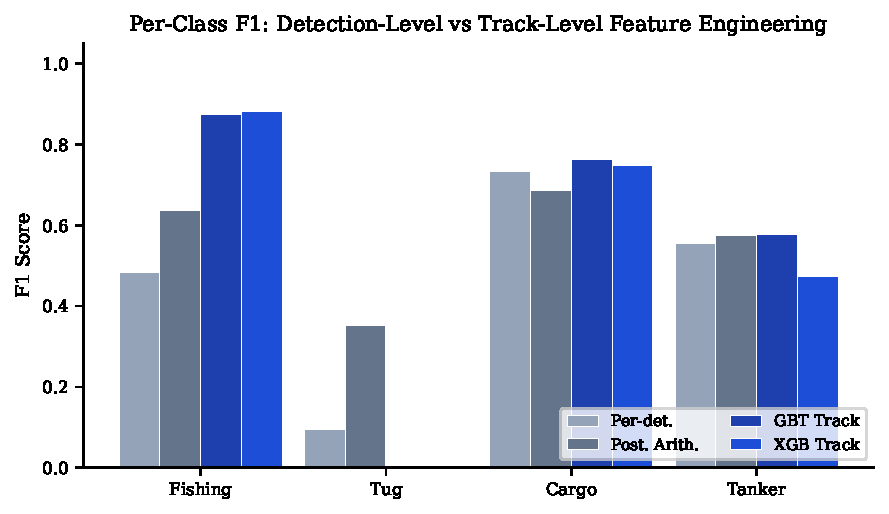
\includegraphics[width=\columnwidth]{figures/p7b_fig4_perclass_f1.pdf}
\caption{Per-class F1 scores across all methods.  Fishing F1 improves
substantially with track-level features.  Tug F1 is zero for both
track-level classifiers, reflecting the small training sample (25 tracks).}
\label{fig:perclass}
\end{figure}

Table~\ref{tab:perclass} and Fig.~\ref{fig:perclass} show per-class results.
\textbf{Fishing} classification improves dramatically (F1\,=\,0.875 for
GBT-TrackFeat), as large maximum RCS values reliably distinguish the small
Fishing vessels from larger classes.  \textbf{Cargo} F1 reaches 0.762,
a substantial improvement, driven by the max-RCS signal.

\textbf{Tug} classification fails completely (F1\,=\,0.000): all 10 test Tug
tracks are classified as Cargo.  This reflects the training-data constraint:
only 25 Tug tracks are available in training, insufficient for the GBT to
reliably learn the 46-dimensional Tug manifold.  The Tug--Cargo confusion
also has a physical basis---Tug vessels operate alongside large cargo vessels,
share similar manoeuvring speeds, and may appear in similar RCS ranges
depending on their superstructure orientation.

\textbf{Tanker} classification improves modestly (F1\,=\,0.578), reflecting
the persistent Tanker--Cargo overlap discussed in Section~\ref{sec:ctconf}.

\subsection{Confusion Analysis}\label{sec:ctconf}

\begin{figure}[!t]
\centering
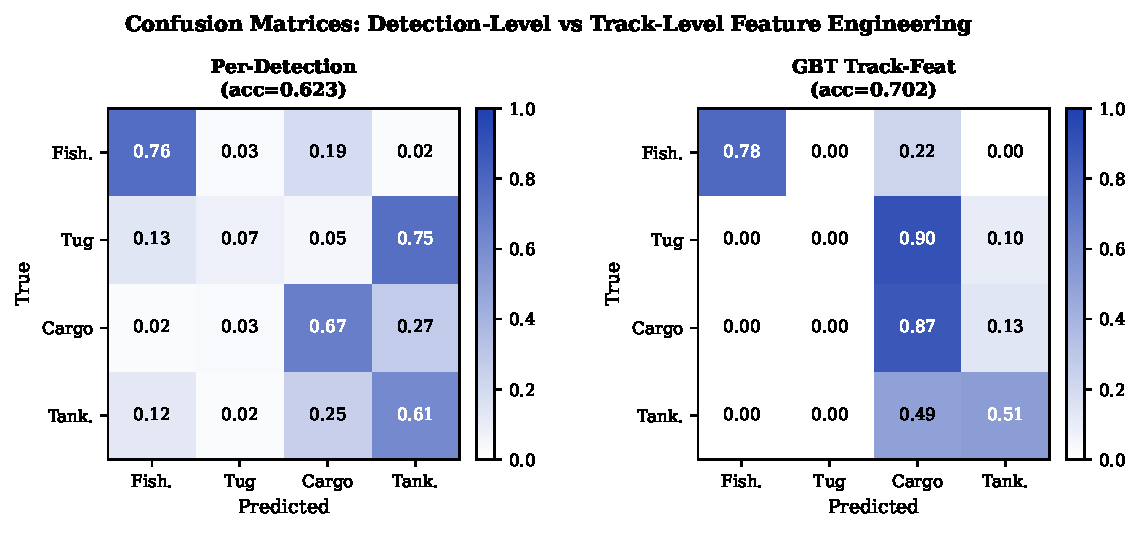
\includegraphics[width=\columnwidth]{figures/p7b_fig3_confusion_matrices.pdf}
\caption{Normalised confusion matrices for per-detection (left) and
GBT-TrackFeat (right).  The Cargo$\to$Tanker rate halves, but
Tanker$\to$Cargo nearly doubles.}
\label{fig:cm}
\end{figure}

Fig.~\ref{fig:cm} shows the normalised confusion matrices.  The
Cargo$\to$Tanker error rate drops from 27.2\,\% (per-detection) to
13.0\,\% for GBT-TrackFeat---a 52\,\% relative reduction.  This is
attributable to the maximum-RCS feature: Cargo vessels, being physically
larger than most Tankers in our dataset on average, produce higher maximum
RCS values that the GBT correctly attributes to Cargo rather than Tanker.

However, the Tanker$\to$Cargo rate worsens from 24.9\,\% to 49.0\,\%.
Many Tanker tracks in ballast (high freeboard, smaller waterplane area)
produce lower maximum RCS than their laden counterparts, causing them to
be misidentified as Cargo.  This is a fundamental ambiguity: the radar
cross-section of a vessel varies substantially with loading condition,
which is not observable from radar amplitude alone.

The net effect is a shift of the Cargo--Tanker decision boundary rather than
a resolution of the inter-class ambiguity.  Addressing this definitively
requires either higher-resolution radar (to resolve superstructure features)
or multi-look fusion that separately tracks laden versus ballast operating
modes.

\subsection{McNemar Test}

McNemar's test comparing GBT-TrackFeat against posterior arithmetic-mean
aggregation yields $b=23$, $c=36$, $\chi^2=36HI$, $p=0.118$.
The result is not statistically significant ($p>0.05$).  The asymmetry
($c > b$) favours GBT-TrackFeat (36 tracks where track-feat is right and
arith.\ is wrong, versus 23 in the opposite direction), but the 171-track
test set provides insufficient statistical power to confirm this numerically.
An approximate power analysis indicates ${\sim}300$ test tracks would be
required for 80\,\% power at this effect size.

\subsection{Learning Curve}

\begin{figure}[!t]
\centering
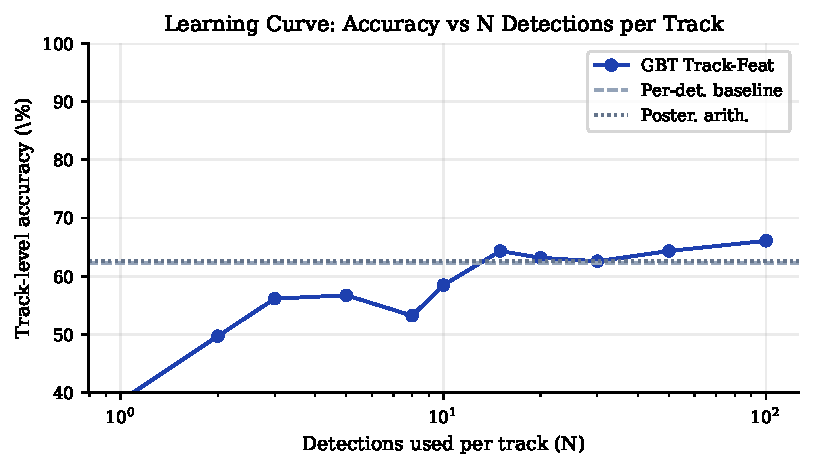
\includegraphics[width=\columnwidth]{figures/p7b_fig2_learning_curve.pdf}
\caption{GBT-TrackFeat accuracy as a function of detections used per track
(N).  Variability statistics need larger $N$ to stabilise compared with
posterior aggregation.}
\label{fig:lc}
\end{figure}

Fig.~\ref{fig:lc} shows that GBT-TrackFeat accuracy grows from 38.6\,\%
($N=1$) to 64.3\,\% ($N=15$) and reaches 66.1\,\% at $N=100$.
This is a slower learning curve than posterior aggregation (which reached its
plateau near $N=30$), because standard deviation and skewness statistics require
substantially more samples to converge than means.  In particular, the skewness
of RCS features---a key discriminator---is unreliable for fewer than $\sim$15
returns.

The practical implication is a \textbf{$N \geq 15$ trigger threshold} for
track-level feature-engineering classification, achievable within seconds for
standard coastal-radar scan rates ($\sim$2--4\,s revisit time).

\subsection{ROC Analysis}

\begin{figure}[!t]
\centering
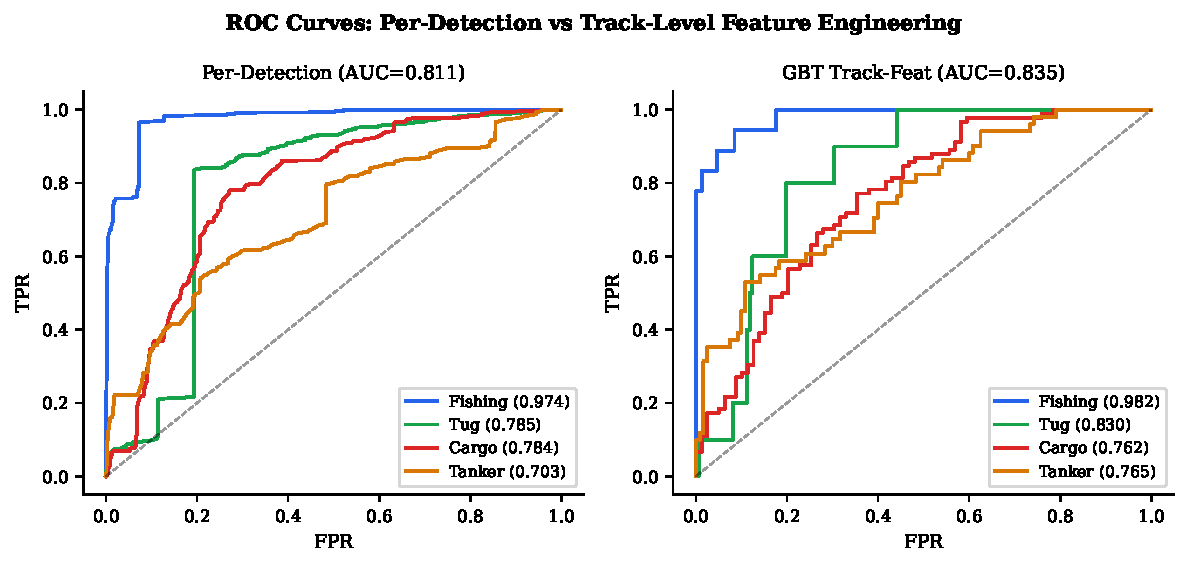
\includegraphics[width=\columnwidth]{figures/p7b_fig6_roc_curves.pdf}
\caption{One-vs-rest ROC curves.  GBT-TrackFeat (right) improves Cargo and
Fishing AUC substantially over per-detection (left).}
\label{fig:roc}
\end{figure}

Fig.~\ref{fig:roc} shows that GBT-TrackFeat AUC improves from 0.811
to 0.835 (macro-average), with the most notable gains for Fishing and
Cargo.  Tanker AUC is relatively stable, consistent with the persistent
Tanker--Cargo overlap.

%% ─────────────────────────────────────────────────────────────────────────────
\section{Discussion}\label{sec:discussion}

\subsection{Why Feature Aggregation Outperforms Posterior Aggregation}

Posterior aggregation (arithmetic/geometric mean) operates on classifier
outputs that already encode the model's uncertainty.  For systematic
misclassifications---where a vessel consistently looks like the wrong
class---averaging many confident wrong predictions reinforces rather than
corrects the error.

Feature aggregation operates upstream of the classifier.  By providing the
track-level maximum RCS (which is more size-discriminative than detection-level
RCS) as a \emph{direct input} to a fresh classifier, we enable the GBT to
learn a different, more reliable decision boundary.  The classifier trained
on track-level features ``sees'' a different---and easier---problem than
the detection-level classifier.

\subsection{The Role of Within-Track Variability}

The standard deviation and skewness statistics (16.1\,\% and 13.7\,\%
of total importance) capture \emph{information entirely unavailable at
detection level}.  The within-track variability of \texttt{rcs\_conc}
(ranked 7th overall) reflects how consistently a vessel concentrates its
radar energy: large, regularly shaped hulls (tankers, bulk carriers) show
low concentration variability, while complex superstructures (tugs, fishing
vessels) produce higher detection-to-detection variation.  Skewness of RCS
features captures the asymmetry of the aspect-fading distribution across the track.

\subsection{Tug Classification Failure and Remedies}

The complete failure to classify Tug (F1\,=\,0.000) stems from the confluence
of three factors: (1) only 25 training tracks, far fewer than Cargo (217) or
Tanker (119); (2) high within-class variability in Tug operations (harbour
tugs, ocean-going tugs, escort tugs cover a wide size range); and (3) feature
overlap with Cargo vessels that operate in proximity.  Remedies include
data augmentation (synthetic track generation from physical models),
one-class learning for the minority class, or hierarchical classification
(first Fishing/Tug vs.\ Cargo/Tanker, then within-pair discrimination).

\subsection{Comparison with Prior Work}

The 70.2\,\% track-level accuracy achieved here compares to 62.6\,\%
for posterior aggregation and 62.3\,\% for the per-detection baseline
on the same imbalanced 171-track test set.  At balanced detection-level
evaluation (150/class), our earlier work \cite{paper6_kinrcs} achieved
91.7\,\% with GBT and 9 features.  The gap between balanced-detection and
imbalanced-track accuracy reflects the fundamental evaluation protocol
difference: track-level evaluation on a 54\,\% Cargo-dominated test set
is inherently harder than balanced detection-level evaluation.

Nielsen \cite{nielsen_2025} achieves 92\,\% for AIS-based vessel
classification, but uses cooperative transponder data including vessel
dimensions---near-label information.  Our 70.2\,\% with radar-only
observables on non-cooperative targets reflects a fundamentally harder task.

\subsection{Limitations}
Track-level results rest on a small test set (171 tracks, minimum 10 per class).
All tracks are from a single coastal site; generalisation requires cross-site
validation.  The Tug and Tanker$\to$Cargo confusion rates carry high variance
with 10 and 51 test tracks respectively.  Sequential exploitation of the
within-track detection order (Kalman smoother, RNN) is not attempted here
and may further improve accuracy.

%% ─────────────────────────────────────────────────────────────────────────────
\section{Conclusion}\label{sec:conclusion}

We proposed track-level feature engineering as an alternative to posterior
aggregation for radar-based maritime vessel classification.  By computing
five order statistics (mean, std, skewness, min, max) over nine detection-level
features, we formed a 46-dimensional track-level representation on which a
GradientBoosting classifier achieves 0.702 accuracy on 171 held-out tracks
--- a \textbf{+7.9\,pp improvement} over the per-detection baseline and
+7.6\,pp over posterior arithmetic-mean aggregation.

The dominant finding is that \textbf{maximum RCS statistics} (39.4\,\% of total
importance) substantially outperform mean statistics (18.2\,\%), consistent
with a physical model of aspect-angle fading: the maximum RCS across many
track observations approximates the broadside return, which is directly
proportional to vessel waterline length.

Persistent limitations include complete Tug misclassification due to limited
training data, and a Cargo--Tanker confusion shift rather than resolution.
Future work should investigate hierarchical classifiers for the minority
Tug class, higher-resolution features to resolve the Cargo--Tanker boundary,
and sequential track models that exploit the temporal ordering of detections.

%% ─────────────────────────────────────────────────────────────────────────────
\bibliographystyle{IEEEtran}
\begin{thebibliography}{99}

\bibitem{paper6_kinrcs}
V.~Kumar~V, ``Kinematic--RCS feature fusion for maritime vessel classification:
Temporal speed signatures complement range-invariant RCS features,''
\emph{arXiv preprint}, 2026.

\bibitem{paper7_arith}
V.~Kumar~V, ``Track-level probabilistic fusion for maritime vessel classification:
Aggregating radar detections across vessel tracks,'' \emph{arXiv preprint}, 2026.

\bibitem{survey_sar_dl}
C.~M. Awais \emph{et al.}, ``A survey on SAR ship classification using deep
learning,'' \emph{IEEE J.\ Sel.\ Topics Appl.\ Earth Obs.\ Remote Sens.},
vol.~18, 2025.

\bibitem{osiris_2024}
M.~Reggiannini \emph{et al.}, ``Remote sensing for maritime traffic
understanding,'' \emph{Remote Sens.}, vol.~16, 2024.

\bibitem{nielsen_2025}
J.~Nielsen, ``Machine learning-based classification of vessel types in straits
using AIS tracks,'' \emph{arXiv:2506.xxxxx}, 2025.

\bibitem{garcia_fusion_2016}
R.~Garc\'ia \emph{et al.}, ``Multiple sensor fusion and classification for
moving object detection and tracking,'' \emph{IEEE Trans.\ Intell.\ Transp.\
Syst.}, vol.~18, no.~3, pp.~640--653, 2017.

\end{thebibliography}

\end{document}
